\section{Mô tả chi tiết}

\subsection{Bối cảnh và vấn đề}
Ngành ngân hàng toàn cầu đang đối mặt với áp lực hiện đại hóa để nâng cao năng lực cạnh tranh và đáp ứng kỳ vọng của khách hàng trong kỷ nguyên số. Tuy nhiên, quá trình này gặp phải nhiều rào cản lớn:
\begin{itemize}
  \item \textbf{Hệ thống truyền thống:} Các hệ thống core banking truyền thống thường cứng nhắc, khó mở rộng và tốn kém để bảo trì, gây khó khăn khi tích hợp công nghệ mới.\cite{haralayya2021core}
  \item \textbf{Chi phí và độ phức tạp:} Việc áp dụng các công nghệ mới như blockchain đòi hỏi chi phí đầu tư lớn và chuyên môn kỹ thuật sâu, đặc biệt là việc tự xây dựng một nền tảng blockchain riêng.\cite{koteska2017blockchain}
  \item \textbf{Bảo mật và tuân thủ:} Các blockchain công cộng phổ biến (permissionless) như Ethereum thường có chi phí giao dịch biến động và không đáp ứng được các yêu cầu khắt khe về tính riêng tư\cite{peng2021privacy}, định danh (KYC/AML) và tuân thủ quy định của Ngân hàng Nhà nước.\cite{Vietnamese2023ND13,Vietnamese2022Luat14,Vietnamese2023ND19,Vietnamese2023TT09}
  \item \textbf{Xu hướng toàn cầu:} Sự ra đời của các sáng kiến blockchain quốc gia như EBSI (European Blockchain Services Infrastructure)\cite{ebsi2020} của Liên minh châu Âu và BSN (Blockchain-based Service Network)\cite{bsn2020} của Trung Quốc cho thấy các cường quốc đang chủ động phát triển hạ tầng blockchain riêng để bảo đảm chủ quyền dữ liệu, thúc đẩy chuyển đổi số và hỗ trợ các dịch vụ công nghệ số hiện đại. Điều này đặt ra yêu cầu cấp thiết để Việt Nam cũng cần có một nền tảng blockchain riêng nhằm không bị tụt hậu trong cuộc đua công nghệ toàn cầu.
\end{itemize}

\subsection{Giải pháp đề xuất: Nền tảng Fichain}
Fichain là một nền tảng blockchain Layer 1 được thiết kế chuyên biệt cho lĩnh vực tài chính - ngân hàng, nhằm giải quyết các rào cản trong quá trình chuyển đổi số:

\begin{itemize}
  \item \textbf{Tối ưu cho hệ thống tài chính:} Fichain cung cấp bộ công cụ và SDK dễ tích hợp với hệ thống core banking hiện có, hỗ trợ các giao diện API linh hoạt, giúp ngân hàng từng bước hiện đại hóa mà không cần thay đổi toàn bộ kiến trúc hiện tại.
  
  \item \textbf{Tiết kiệm chi phí và đơn giản hóa triển khai:} Fichain cung cấp một hạ tầng blockchain hoàn chỉnh dưới dạng dịch vụ (Blockchain-as-a-Service), giúp ngân hàng tránh được chi phí đầu tư ban đầu lớn và gánh nặng vận hành, đồng thời được hỗ trợ kỹ thuật chuyên sâu.
  
  \item \textbf{Tuân thủ pháp lý và bảo mật dữ liệu:} Fichain hỗ trợ cơ chế định danh, phân quyền truy cập (permissioned blockchain) và lưu trữ dữ liệu theo chuẩn trong nước, bảo đảm tuân thủ các quy định về bảo mật, KYC/AML và các nghị định liên quan của Ngân hàng Nhà nước.
  
  \item \textbf{Phù hợp với xu hướng quốc tế:} Tương tự như EBSI của châu Âu hay BSN của Trung Quốc, Fichain hướng đến mục tiêu xây dựng một hạ tầng blockchain quốc gia cho Việt Nam, nhằm bảo vệ chủ quyền dữ liệu, nâng cao năng lực số hóa ngành ngân hàng, và hỗ trợ phát triển các dịch vụ công nghệ tài chính hiện đại.
\end{itemize}

Với Fichain, các tổ chức tài chính tại Việt Nam không chỉ có cơ hội nâng cấp hạ tầng theo tiêu chuẩn quốc tế, mà còn góp phần chủ động tham gia vào hệ sinh thái số của quốc gia trong tương lai.

\subsection{Công nghệ cốt lõi}
Nền tảng Fichain được xây dựng từ gốc để đáp ứng các yêu cầu đặc thù của ngành tài chính.
\begin{itemize}
    \item \textbf{Native Coin là Việt Nam Đồng (VNĐ):} Một trong những khác biệt lớn nhất của Fichain là việc sử dụng đồng Việt Nam làm đơn vị tiền tệ gốc của mạng lưới. Về bản chất, đây là một dạng stablecoin được bảo chứng 1:1 với tiền pháp định (fiat). Điều này mang lại các lợi ích then chốt:
    \begin{itemize}
        \item Loại bỏ hoàn toàn biến động giá trị, vốn là rủi ro lớn nhất khi dùng các crypto-asset thông thường trong nghiệp vụ ngân hàng.
        \item Đơn giản hóa việc hạch toán, báo cáo và đối soát cho các tổ chức tài chính.
        \item Giúp người dùng cuối dễ dàng hiểu và tiếp cận, vì mọi giao dịch đều được định giá bằng đơn vị tiền tệ quen thuộc.
    \end{itemize}
    
    \item \textbf{Cơ chế đồng thuận PoSA (Proof of Staked Authority):} Đây là cơ chế lai kết hợp giữa PoA và PoS. Các validator (nút xác thực giao dịch) không chỉ phải được định danh và có uy tín (Authority - ví dụ: các ngân hàng trong liên minh) mà còn phải ký quỹ một lượng tài sản lớn (Stake). Mô hình này đảm bảo hiệu suất cao, bảo mật cấp doanh nghiệp và khả năng phân quyền có kiểm soát.

    \item \textbf{Tương thích EVM (Ethereum Virtual Machine):} Hỗ trợ đầy đủ EVM cho phép các nhà phát triển dễ dàng triển khai các hợp đồng thông minh (smart contract) viết bằng Solidity và các ứng dụng phi tập trung (DApps) từ hệ sinh thái Ethereum rộng lớn.
    
    \item \textbf{Mô hình mạng linh hoạt:} Fichain có thể được triển khai dưới dạng mạng riêng tư (private) cho một tổ chức, hoặc mạng liên minh (consortium) cho nhiều đối tác, đảm bảo tuân thủ các quy định về dữ liệu và bảo mật.
\end{itemize}

\subsection{Kiến trúc hệ thống}
Kiến trúc của Fichain được chia thành năm lớp chính, mỗi lớp đảm nhiệm một vai trò cụ thể trong hệ thống. Sơ đồ tổng quan được thể hiện trong Hình~\ref{fig:architecture}.

\begin{figure}[h!]
    \centering
    % The image architecture.png should be placed in the specified path.
    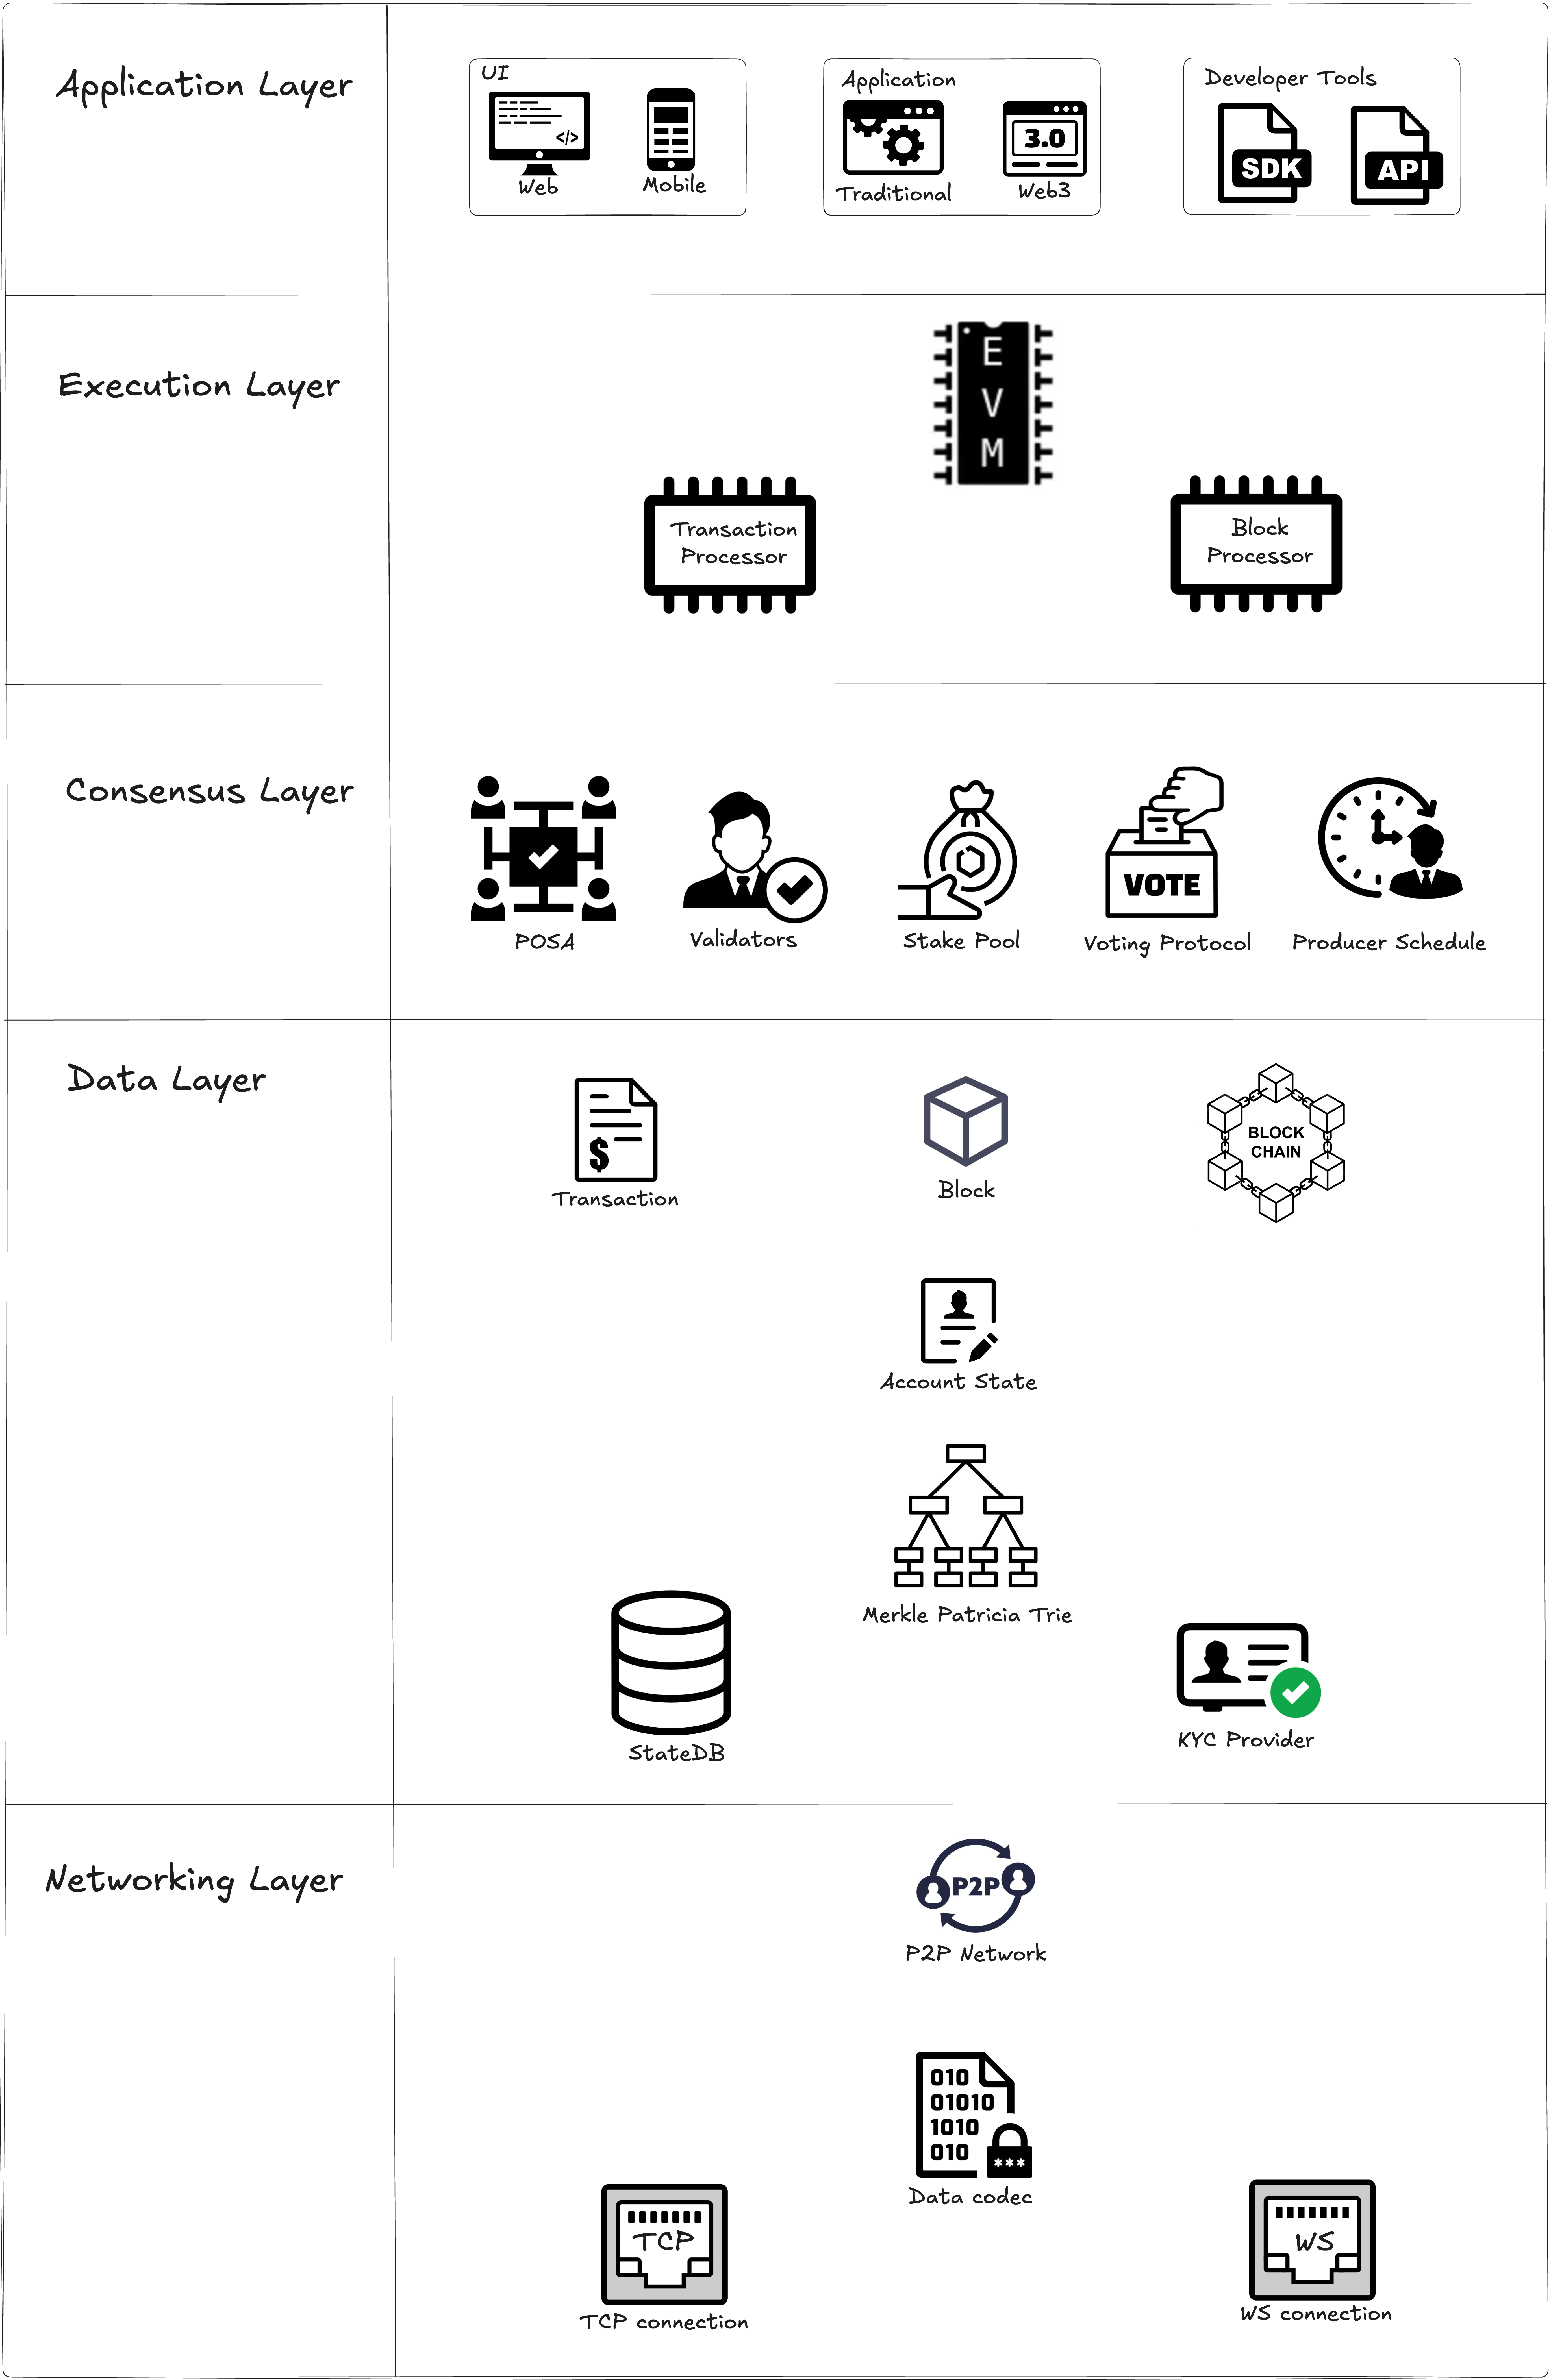
\includegraphics[width=0.9\textwidth]{architecture.png} 
    \caption{Sơ đồ kiến trúc các lớp của Fichain.}
    \label{fig:architecture}
\end{figure}

\begin{itemize}
    \item \textbf{Lớp Ứng dụng (Application Layer):} Đây là lớp giao tiếp trực tiếp với người dùng cuối và nhà phát triển. Nó bao gồm giao diện người dùng (UI) cho Web và Di động, các ứng dụng (Truyền thống và Web3), và các công cụ dành cho nhà phát triển như SDK và API để xây dựng và tích hợp các ứng dụng phi tập trung (DApps).

    \item \textbf{Lớp Thực thi (Execution Layer):} Chịu trách nhiệm xử lý logic của hệ thống. Lớp này chứa Máy ảo Ethereum (EVM) để thực thi các hợp đồng thông minh, cùng với Bộ xử lý Giao dịch (Transaction Processor) và Bộ xử lý Khối (Block Processor) để xử lý và xác thực các hoạt động trên chuỗi.

    \item \textbf{Lớp Đồng thuận (Consensus Layer):} Đảm bảo tính toàn vẹn và nhất quán của toàn mạng lưới. Fichain sử dụng cơ chế đồng thuận PoSA (Proof of Staked Authority), trong đó các Validators được chọn để tạo khối mới. Lớp này cũng bao gồm các thành phần như Bể khoá cọc(Stake Pool), Giao thức Bỏ phiếu (Voting Protocol) và Lịch trình sản xuất khối (Producer Schedule).

    \item \textbf{Lớp Dữ liệu (Data Layer):} Quản lý việc lưu trữ tất cả dữ liệu của chuỗi khối. Các thành phần chính bao gồm cấu trúc của Giao dịch (Transaction), Khối (Block) và toàn bộ Chuỗi khối (Blockchain). Lớp này cũng quản lý Trạng thái tài khoản (Account State), sử dụng cây Merkle Patricia Trie để đảm bảo tính toàn vẹn dữ liệu, lưu trữ trạng thái trong StateDB, và có thể tích hợp với Nhà cung cấp KYC.

    \item \textbf{Lớp Mạng (Networking Layer):} Quản lý việc giao tiếp giữa các nút (nodes) trong mạng lưới. Lớp này hoạt động trên một mạng ngang hàng (P2P Network), sử dụng các giao thức kết nối như TCP và WebSocket (WS), và một bộ mã hóa/giải mã dữ liệu (Data codec) để truyền thông tin một cách an toàn và hiệu quả.
\end{itemize}
